% 1993_旧科目组_文科/figures/f1993_old_arts_q18_cube.tex — 1993 年·旧科目组·文科，第 18 题正方体与中点连线
%
% 【来源】`.work/phase4-b18/source/1993旧科目组文.pdf`（SHA-256 c8e57edcf61e754a36e9b5775c40d9277e0c3f45cb0f93b478118c5cb2219f86），第 1 页；
%   内容流逐路径照录，本地坐标 = 页面坐标 − (558.620,319.619)，1 单位 = 1 TeX pt。
%   线宽 0.398pt；虚线 [2.989 2.989] 0 d。
%
% 标签微调：D₁ 左上移 (-1.0,1.5)pt、B₁ 右上移 (1.0,1.0)pt，避开顶点与隐藏棱
% 元素计数：实线 9 段＋虚线 5 段（3 条不可见棱＋CM、D₁N）＋10 个标签
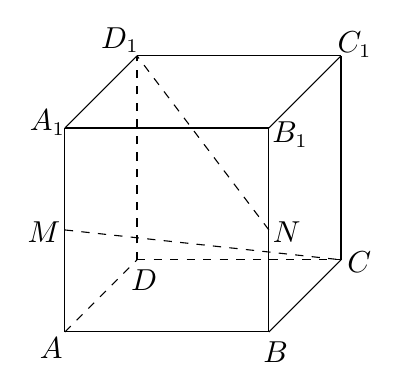
\begin{tikzpicture}[x=1pt, y=1pt,
    every node/.style={inner sep=0pt, font=\fontsize{10.5pt}{12.6pt}\selectfont}]
  \draw[line width=0.398pt] (0.000,0.000) -- (73.703,0.000);
  \draw[line width=0.398pt] (99.758,26.054) -- (73.703,0.000);
  \draw[line width=0.398pt] (0.000,73.703) -- (73.703,73.703);
  \draw[line width=0.398pt] (73.703,0.000) -- (73.703,73.703);
  \draw[line width=0.398pt] (0.000,0.000) -- (0.000,73.703);
  \draw[line width=0.398pt] (99.758,99.758) -- (73.703,73.703);
  \draw[line width=0.398pt] (99.758,99.758) -- (26.054,99.758);
  \draw[line width=0.398pt] (0.000,73.703) -- (26.054,99.758);
  \draw[line width=0.398pt] (99.758,99.758) -- (99.758,26.054);
  % 虚线：不可见棱与题设连线
  \draw[line width=0.398pt, dash pattern=on 2.989pt off 2.989pt] (26.054,26.054) -- (99.758,26.054);
  \draw[line width=0.398pt, dash pattern=on 2.989pt off 2.989pt] (26.054,26.054) -- (26.054,99.758);
  \draw[line width=0.398pt, dash pattern=on 2.989pt off 2.989pt] (0.000,36.852) -- (99.758,26.054);
  \draw[line width=0.398pt, dash pattern=on 2.989pt off 2.989pt] (73.703,36.852) -- (26.054,99.758);
  \draw[line width=0.398pt, dash pattern=on 2.989pt off 2.989pt] (0.000,0.000) -- (26.054,26.054);
  \node[anchor=center] at (19.880,105.381) {$D_1$};
  \node[anchor=center] at (104.680,103.881) {$C_1$};
  \node[anchor=center] at (-6.320,75.581) {$A_1$};
  \node[anchor=center] at (81.380,71.281) {$B_1$};
  \node[anchor=center] at (-7.550,36.001) {$M$};
  \node[anchor=center] at (106.360,25.201) {$C$};
  \node[anchor=center] at (-4.930,-5.779) {$A$};
  \node[anchor=center] at (80.110,36.001) {$N$};
  \node[anchor=center] at (28.580,18.761) {$D$};
  \node[anchor=center] at (76.110,-7.299) {$B$};
\end{tikzpicture}
%
% 【自验结果】坐标逐点照录内容流；标签取 pdftotext -bbox 中心（字母与下标合并取中点）。
